\label{DL_theory}
\section{Deep Learning for spectroscopic data}

Techniques of machine learning and deep learning specifically have been applied to spectroscopic data since the 1990s. It has been applied to a variety of spectroscopic methods such as Near Infrared Spectroscopy (NIR), Raman Spectroscopy, Nuclear Magnetic Resonance Spectroscopy (NMR) and Infrared Spectroscopy (IR) . However, chemometric or physics-based approaches have been and still are favored for data analysis due to the lack of model explainability for data-driven approaches. To oppose, chemometrics is most often based on decomposition techniques such as Principal Component Analysis (PCA) and subsequent linear regression - which inherently does not meet the requirements for explainability.

Deep learning has been previously applied to XPS-analysis by Drera et al.\cite{drera_deep_2019}. They achieved an overall performance of quantitative detection above 10$\%$ content, similar to the detection limit of users - they state. They used solely convolutional neural networks to build their prediction model. Their training data was constructed similarly to the data used in this work. Moreover, Hunt investigated depth profiling using XPS in combination with the singular value decomposition (SVD) algorithm \cite{hunt_depth_2000}. Additionally, Hunter modelled the impact of sample surface roughness on the prediction using the SVD algorithm and the Tyler regularization algorithm.

Attention-based neural networks have been applied to near infrared spectroscopy analysis of medical fungi \cite{huang_attention_2019} and sand gravel \cite{yuan_hybrid_2022} to successfully identify secondary parameters, such as moisture or polysaccharide content with similar or better results than the well-known partial least squares (PLS) fitting.

% advances in DL & applications to spectroscopy tasks
\subsection{Model hyperparameters \& training}
For each model, a set of hyperparameters define either initial, or fixed values used for the training. 
Multiple training cycles are performed on the dataset, which is shuffled before each training cycle, also called epoch. A so-called \emph{loss function} is introduced which resembles the absolute deviation of the predicted $\hat{y}$ from the correct labels $y$ $(\hat{y} - y)$.
In each epoch, we re-evaluate the weights of the model subject to minimize the defined loss-function with respect to the defined learning rate. The initial data available is split into a training and validation dataset. The weights are trained only the training dataset, while the validation dataset is used to check the performance on data which is new for the model and tune its hyperparameters.

\subsection{General patterns}


\subsubsection{Dense layers}
What is often referred to as fully connected, dense, feed-forward neural network or Multilayer Perceptron describes a network consisting of solely fully connected layers. These layers are connected in an $n:m$ manner, where each node of a layer with $n$ nodes is connected with each node of a layer with $m$ nodes. 

\subsubsection{Dropout}
Dropout layers are often used to regularize and generalize models. In these layers, which are fully connected layers, a certain percentage of nodes are not used during training and the specific unused nodes are selected from new each training cycle. This ensures that the training of the network does not rely on only a subset or even a single node, but on all nodes in a similar intensity. The fraction of nodes defined to drop each training cycle is denoted as $p$.

\subsubsection{Batch-Normalization}
Big datasets are usually divided into subsets such that we can efficiently train our network. This is done because the data might not fit the available computing memory and thus slow our computation. Additionally, we train on a subset because finding the global optimum is much more difficult than finding it for the so-called batch. However, even if we randomly split the dataset, we will encounter a non-uniform distribution of information between our batches. Thus, in a batch-normalization layer, each batch input is normalized to have a mean of zero and a standard deviation of one. 
%The positive effects have been shown in multiple publications

\subsection{Convolutional Neural Networks (CNN)}
In convolutional neural networks (CNN), the input values are multiplied with a kernel to extract features. The CNNs are used where the input is of a discrete, grid-like topology. A kernel in this sense can represent a vector of n dimensions, where in case of spectra n=1 that will be moved along an axis, applying the multiplication subsequently. The values of the kernel are learnable, such that it can be fitted to extract specific features depending on the nature of the data.

These convolutional layers are usually followed by pooling layers - such as max-pooling or average-pooling - which also use a kernel. As the pooling layers reduce the dimensionality of the input, they have a number of positive effects on the model, such as better robustness to input variability and faster training. In addition, pooling layers help the model to learn invariances in the input data, such as rotation or small shift of an image content \cite{goodfellow_deep_2016}. 

The 1-dimensional convolutions we use in the case of spectral data will thus use $p$ one-dimensional kernels (vectors) of pre-defined length, where $p$ stands for the number of channels. If, for example, our spectrum vector is of dimensions (1 x 1024), using a 1d-convolutional kernel of size (1 x 5) with 16 channels will be applied. Thus, we will retain 16 vectors of size (1023)

This network architectural pattern is extensively used in image classification tasks but has also been applied to diverse classification tasks, including spectroscopic data analysis \cite{sun_cnnlstm_2023, castorena_deep_2021, drera_deep_2019}.

\subsection{Residual networks}

In residual networks, the input is re-added after performing weighted operations such as convolutions. This feature has known positive effects, especially on deeper neural networks (networks with multiple layers). Residual network architectures diminish the well-known vanishing gradient problem by adding skip connections to the network. 

\begin{figure}[H]
    \centering
    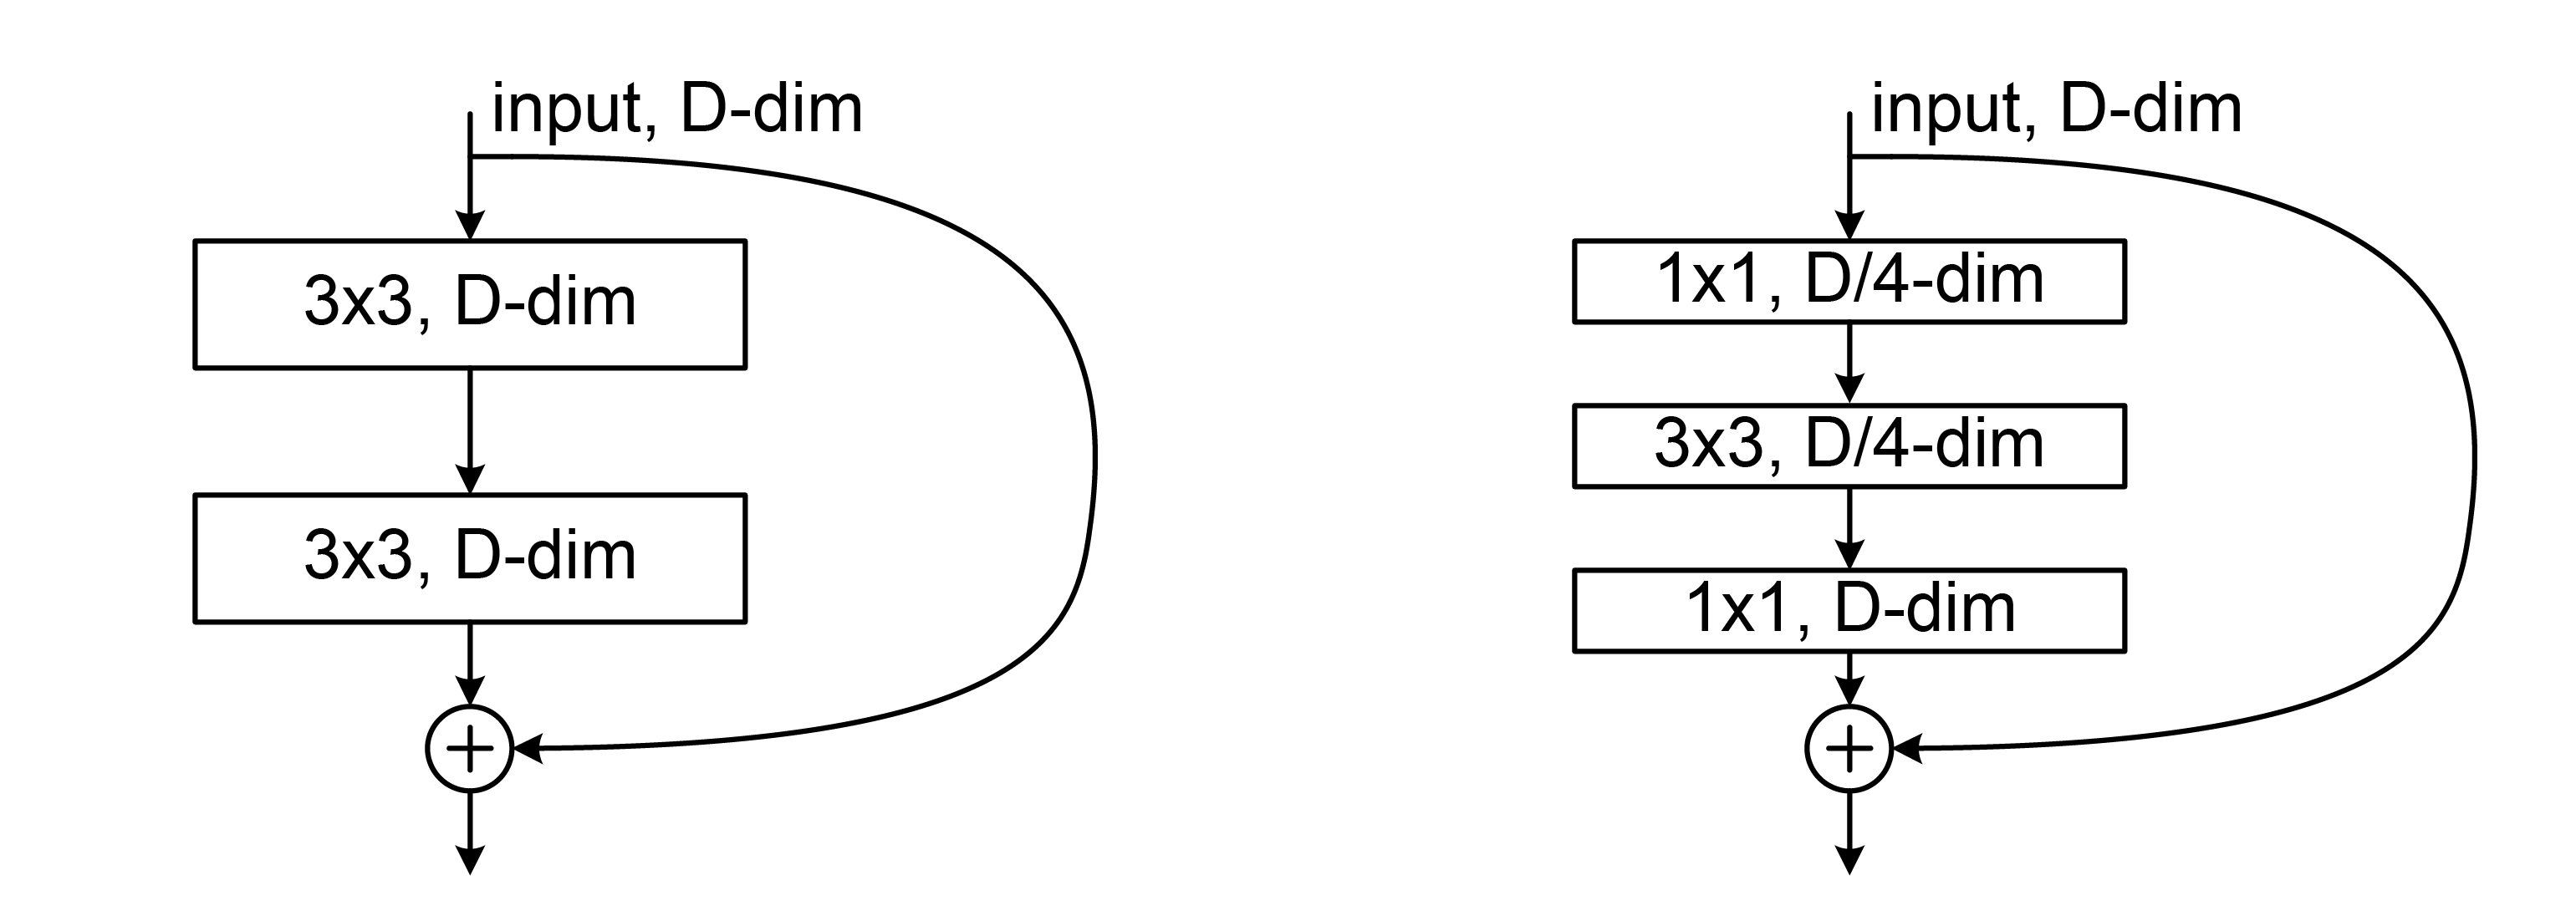
\includegraphics[width=0.5\textwidth]{Figures/ResBlockVariants.png}
    \caption{Residual block pattern}
    \label{fig:res_block}
\end{figure}

This pattern has later also been used for other models, as it allows much deeper networks to learn much more efficiently.

%\subsection{Recurrent neural networks}
    
%In recurrent neural networks (RNNs), temporal information is kept in a hidden representation vector. Because of this temporal representation, RNNs are specialized for processing sequences, such as text. The input information is fed sequentially and the representation vector changes its state. This allows the model to learn 

\subsection{Transformer-based networks}

Originally developed to solve neural language processing (NLP) tasks, the attention mechanism was first described in 2017 \cite{vaswani_attention_2023}.
The combination of an encoder-decoder paradigm with the Multi-Head Attention architecture lead to the development of the Transformer model. The most recent architecture used for NLP tasks is shown in \nameref{fig:transformer_model}.
A transformer consists of tokenizers, embedding layers and transformer layers which include the Attention layers and Multilayer perceptron layers.

\begin{figure}[H]
    \centering
    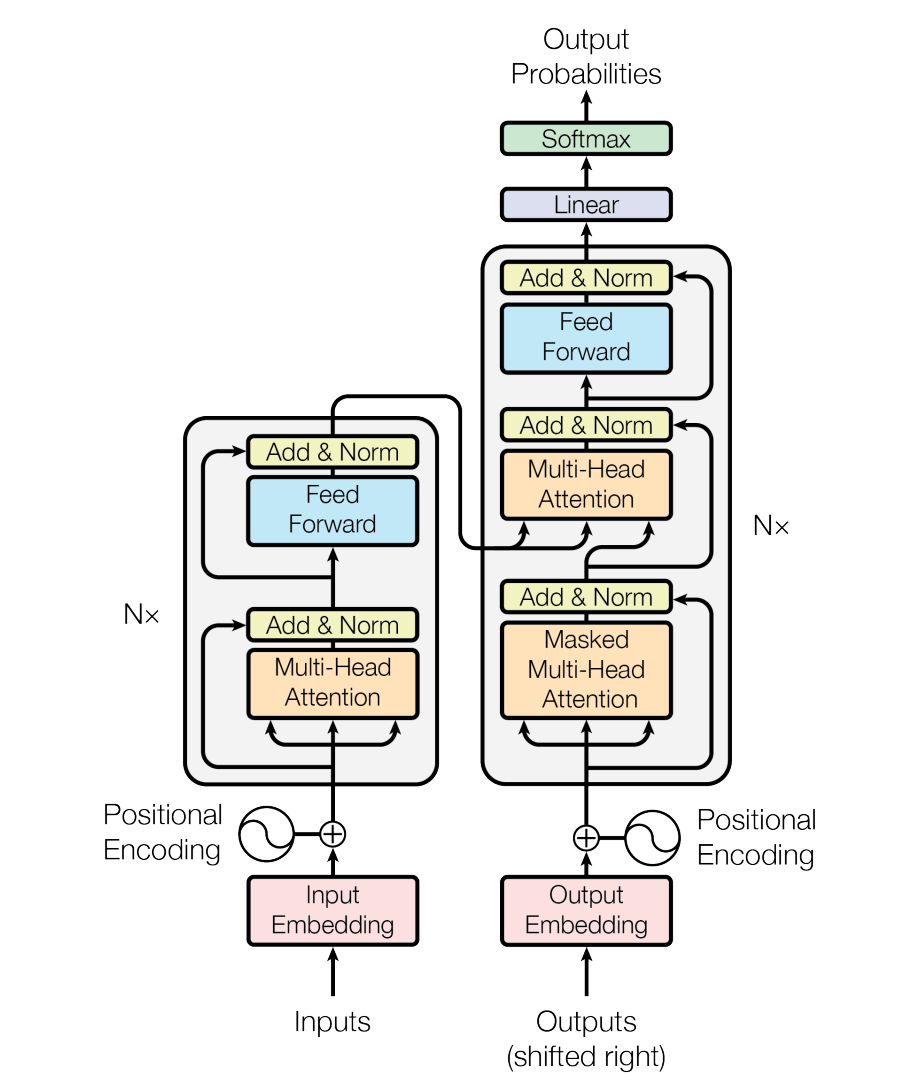
\includegraphics[width=0.6\textwidth]{Figures/Transformer.png}
    \caption{The Transformer-model architecture \cite{vaswani_attention_2023}}
    \label{fig:transformer_model}
\end{figure}

The positional embedding ensures that the model can interpret the position of the tokens within the sequence. The Multi-Head Attention block consist of linear mappings of query, key and value pairs which are run in parallel. The number of linear mappings computed per block is denoted as $h$. Thus, the attention function is performed on a set of queries and an attention matrix is computed \cite{vaswani_attention_2023}.

\subsubsection{Convolutional Block Attention Module (CBAM)}
The Convolutional Block Attention Module (CBAM) connects the attention paradigm with the convolutional approach and mainly consists of two sub-modules. Inputs are taken and with the first module, a 1D channel attention map is generated. Afterwards, these channel attentions are used as an input to the spatial attention module to compute the spatial attention. These two blocks can then be integrated within a convolutional based network or a residual based network.

\begin{figure}[H]
    \centering
    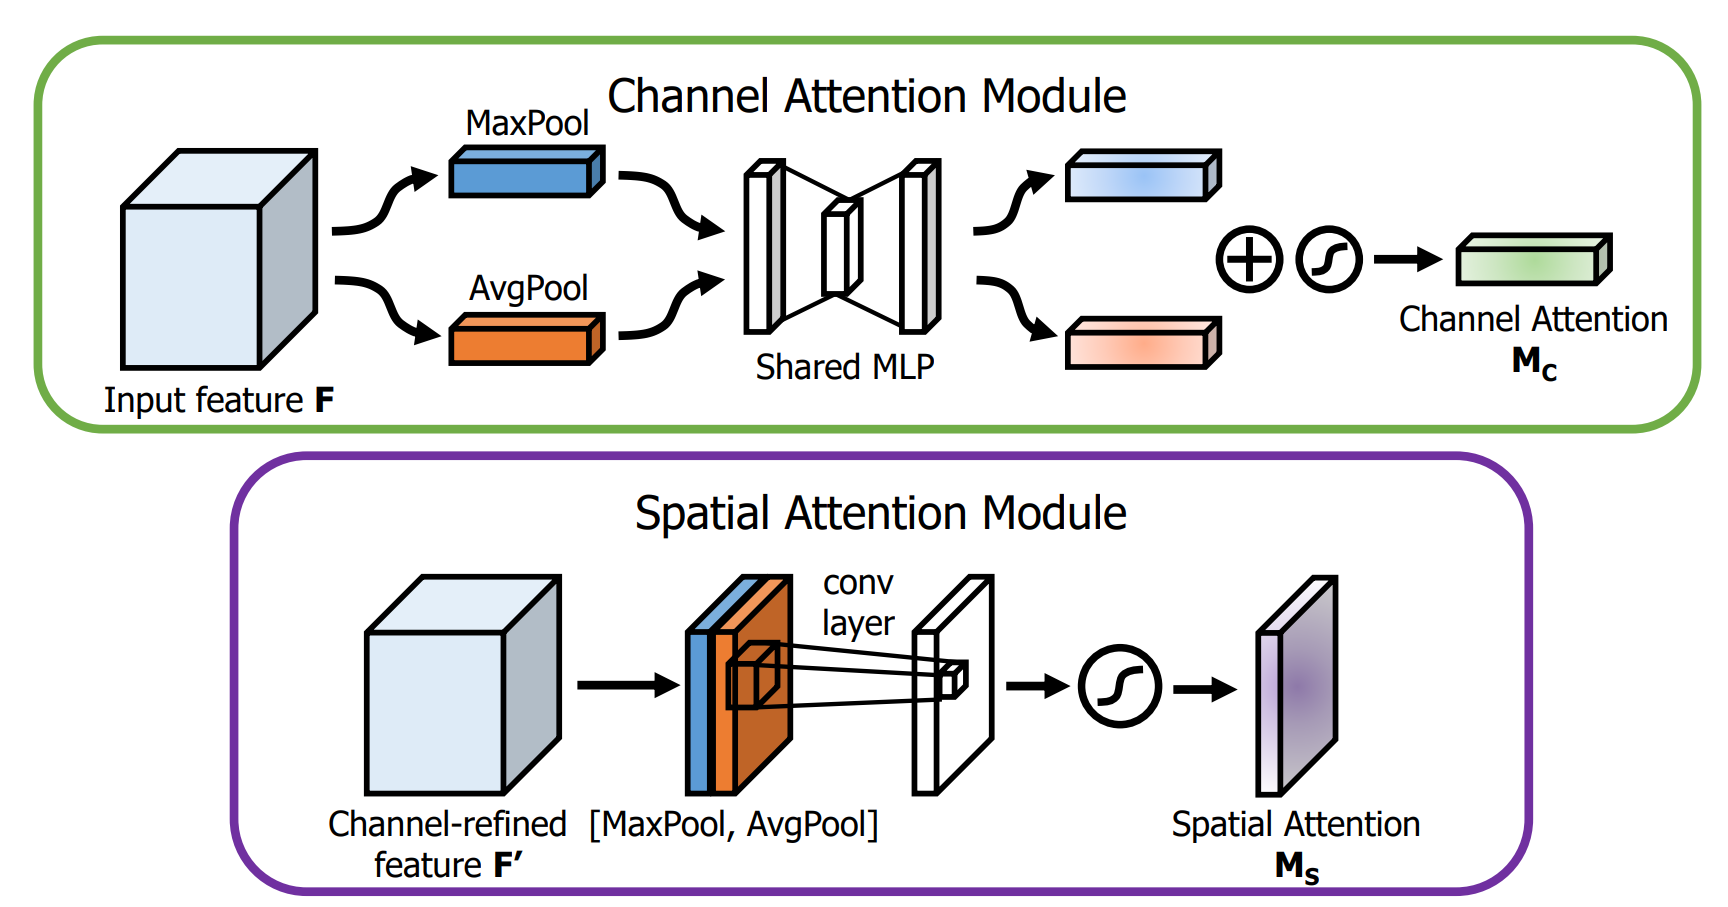
\includegraphics[width=\textwidth]{Figures/cbam_modules.png}
    \caption{Channel \& spatial attention module blocks \cite{woo_cbam_2018}}
    \label{fig:cbam_modules}
\end{figure}

\begin{figure}[H]
    \centering
    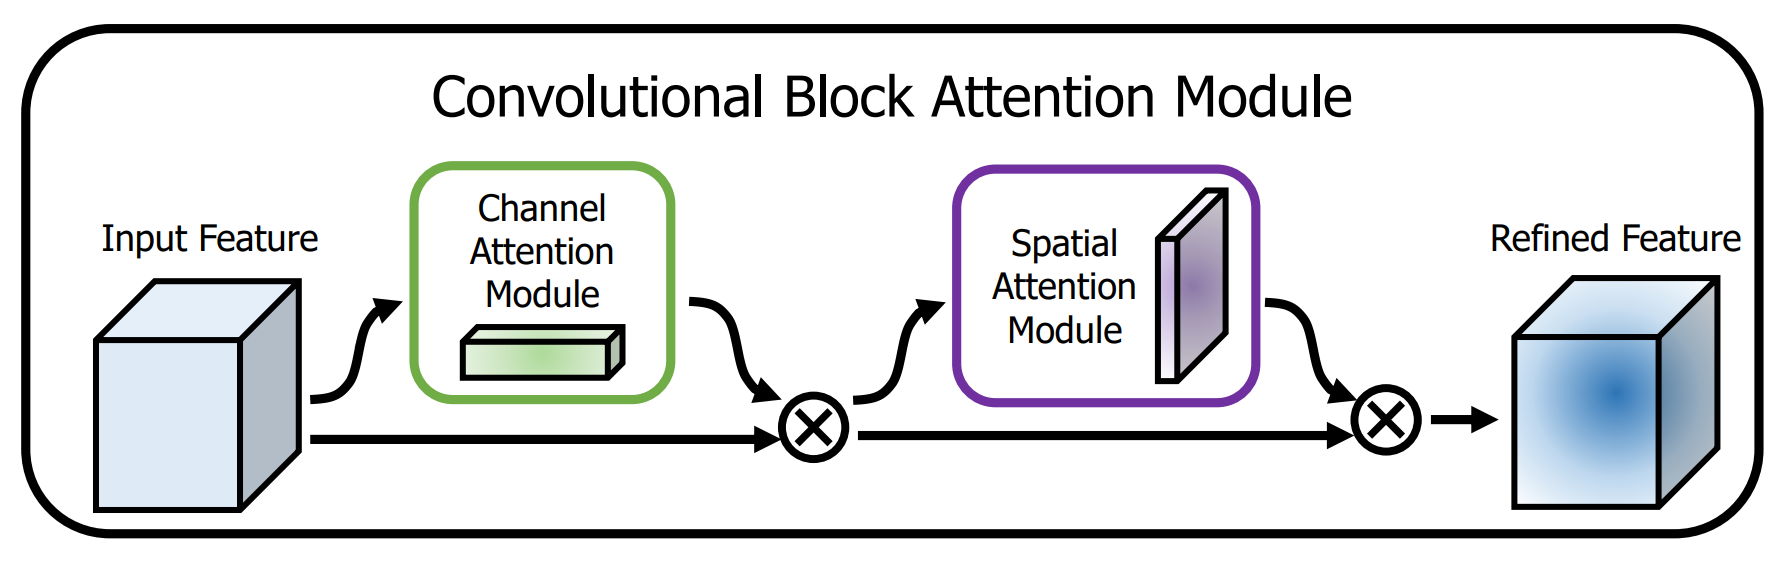
\includegraphics[width=0.7\textwidth]{Figures/cbam_modul.png}
    \caption{CBAM-architecture \cite{woo_cbam_2018}}
    \label{fig:cbam}
\end{figure}


\subsubsection{Vision Transformer (ViT)}
The Vision transformer model (ViT) has been recently published \cite{dosovitskiy_image_2021} and uses the mechanisms of Transformer-based models for computer vision tasks. Input data is divided into multiple patches of size n. A positional embedding is added and the embedded patches are then used as tokenized input to the transformer encoder. 
\begin{figure}
    \centering
    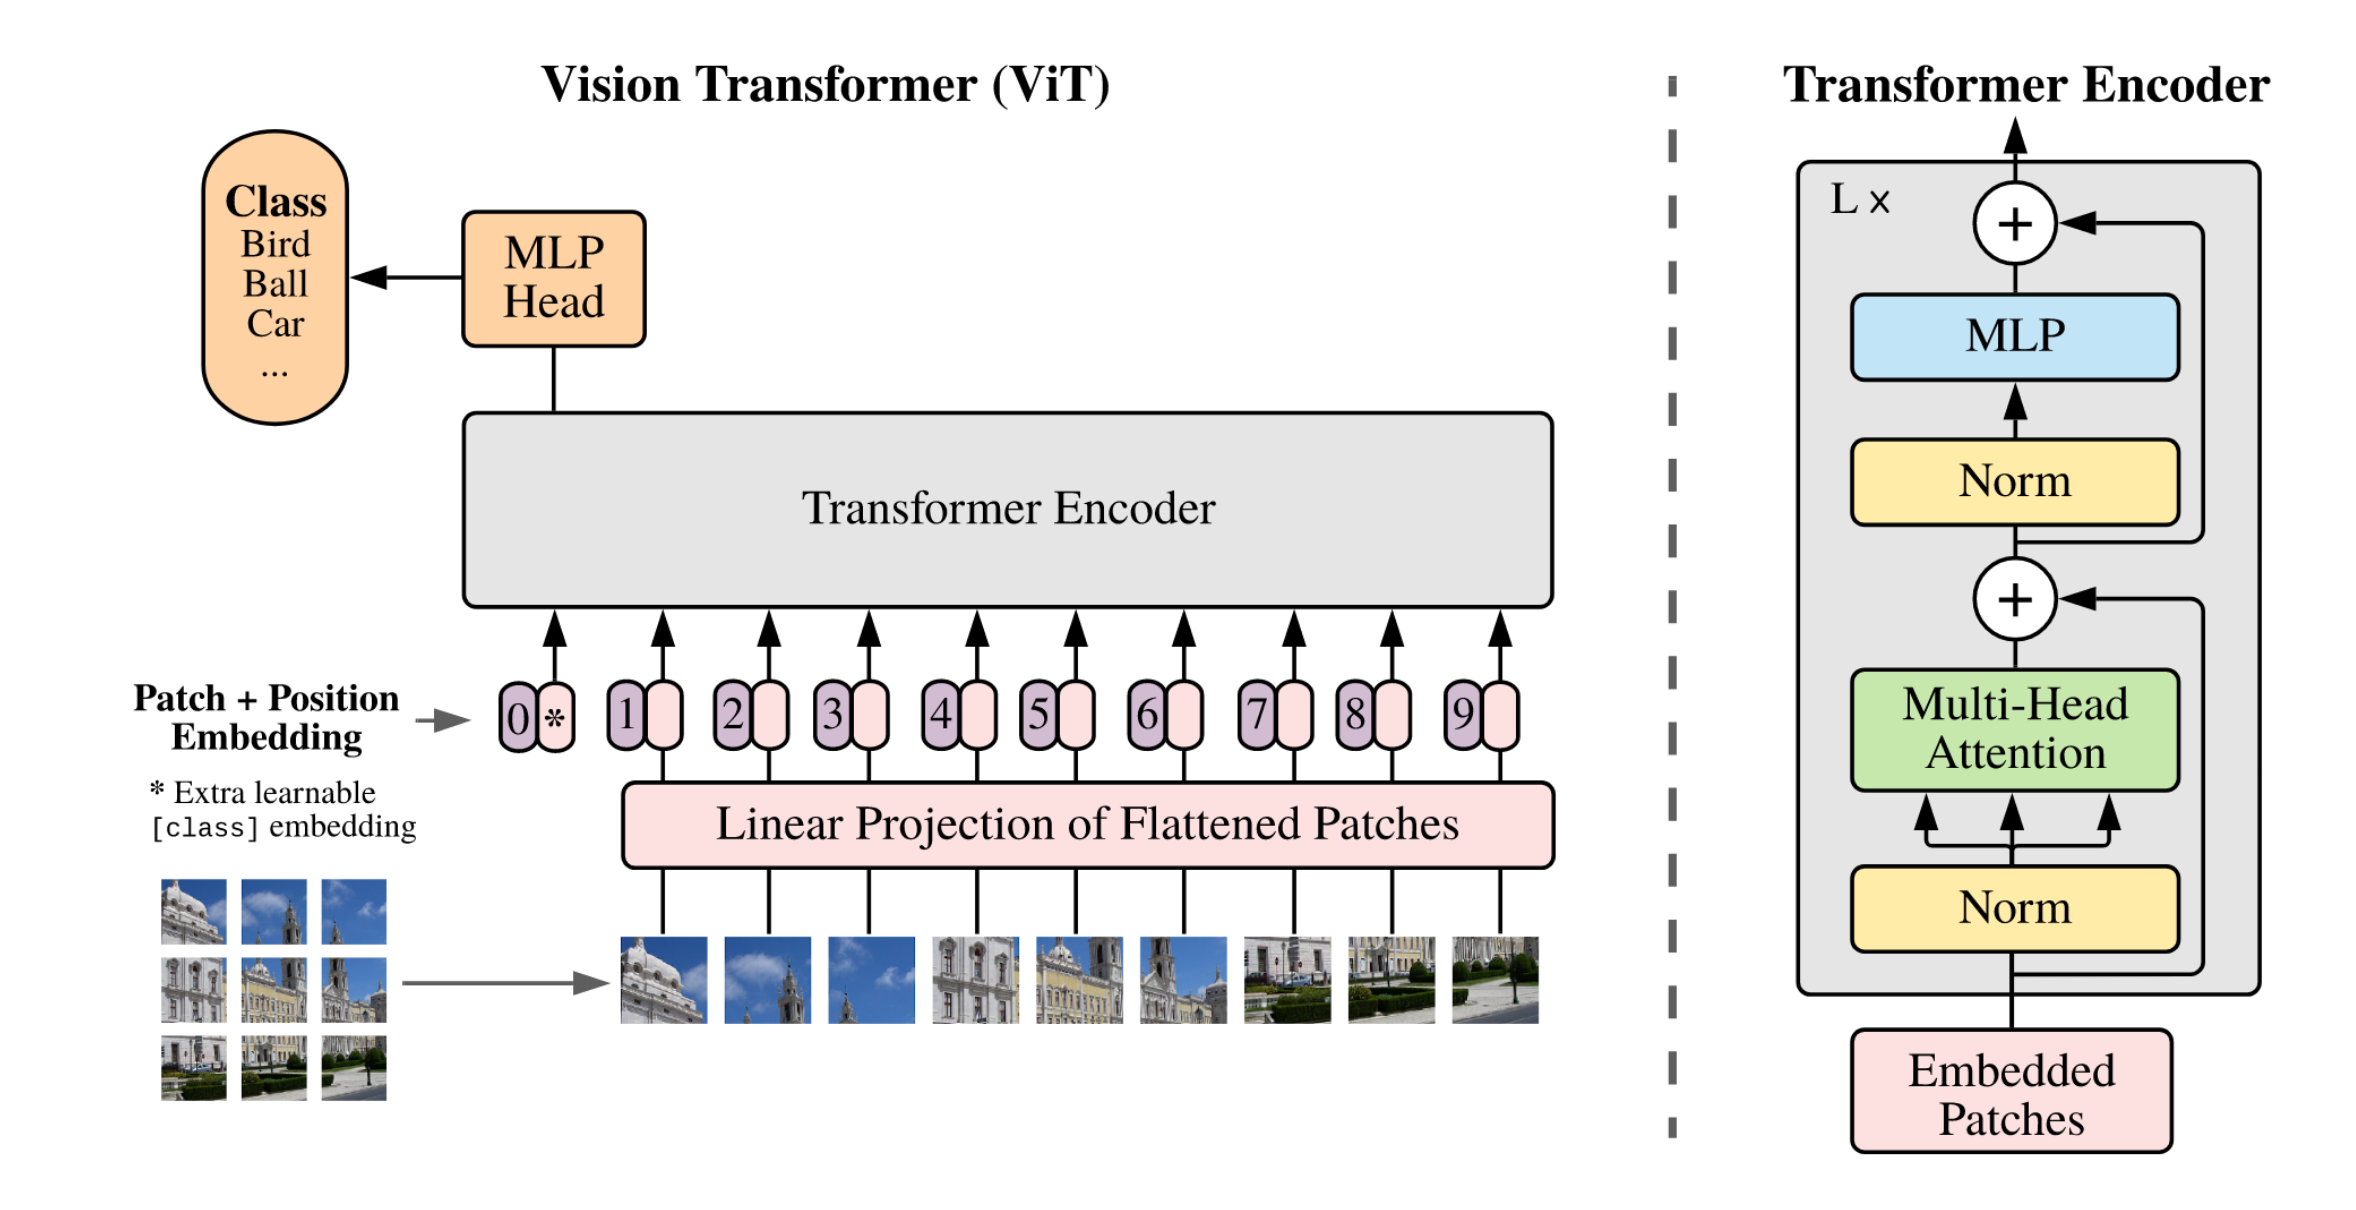
\includegraphics[width=\textwidth]{Figures/ViT.png}
    \caption{Vision Transformer \cite{dosovitskiy_image_2021}}
    \label{fig:vit_model}
\end{figure}
